\section{Basal Boundary Condition}
This section describes the formulation of the basal boundary condition.
An interface for the upper boundary condition (atmospheric BC) is easily defined by the surface temperature and mass balance. Similarly, the basal boundary consists of mechanical and thermal boundary conditions. The complications arise because the thermal and mechanical boundary conditions depend on each other. The interface of the basal boundary can be described with the following fields (see also Fig. \ref{num.fig.basal_bc}):
\begin{enumerate}
\item \textbf{basal traction:} This field specifies a parameter which is used to allow basal sliding.
\item \textbf{basal heat flux:} This is the heat flux entering the ice sheet from below.
\item \textbf{basal water depth:} The presence of basal melt water affects the basal ice temperature.
\end{enumerate}
Also, the ice sheet model calculates a melt/freeze rate based on the temperature gradient and basal water depth. This is handled by Glide.

\begin{figure}[htbp]
  \centering
  
\includegraphics[width=0.9\textwidth]{\dir/figs/basal_bc.eps}
  \caption{Basal boundary condition.}
  \label{num.fig.basal_bc}
\end{figure}

\subsection{Mechanical boundary conditions}
If the ice is not frozen to the bed, basal d\'{e}collement may occur. This can be parameterized by a traction factor, $t_b$. 
Within the ice sheet model, $t_b$ can be used to calculate basal sliding velocities $\vec{u}_b$ in the case of zero--order physics. That is,
\begin{equation}
  \vec{u}_b=t_b\vec{\tau}_b,
\end{equation}
where $\tau_b$ is the basal shear stress. Alternatively, $t_b$ can be used as part of the stress--balance calculations when the model is used with higher order physics. In simple models $t_b$ may be uniform or prescribed as a spatial variable. More complex models may wish to make $t_b$ dependent on other variables, such as basal melt rate. Typically $t_b$ will depend on the presence of basal water.

The second mechanical boundary condition, basal melting/freeze--on $M_b$, is handled within the ice sheet model. The details are described in Section \ref{num.sec.bc_melt}.

\subsection{Thermal boundary conditions}
\label{sc:glide_thermal_bc}
The thermal boundary condition at the ice base is more complicated than the mechanical BC. The ice is heated from below by the geothermal heat flux. Heat is generated by friction with the bed. Furthermore, the ice temperature is constrained to be less than or equal to the pressure melting point of ice. The thermal boundary condition is a flux condition if there is no water present. If there is water, the basal temperature is set to the pressure melting temperature. (If it were lower, there would be no water, and if it were higher, there would be no ice.)

\subsubsection{Basal melting and freezing}\label{num.sec.bc_melt}
At the ice base, $z=b$, we can define outgoing and incoming heat fluxes, $H_o$ and $H_i$:
\begin{subequations}
  \begin{align}
    H_o&=-k_{\text{ice}}\left.\frac{\pd T}{\pd z}\right|_{z=b^+}\\
    \intertext{and}
    H_i&=-k_{\text{rock}}\left.\frac{\pd T}{\pd z}\right|_{z=b^-}+\vec{u}_b\cdot\vec{\tau}_b+
    \begin{cases}
      {\rho_{\text{ice}}M_b}/{L} & \text{when $M_b<0$} \\
      0 & \text{otherwise}
    \end{cases}
  \end{align}
\end{subequations}
where $k_{\text{ice}}$ and $k_{\text{rock}}$ are the thermal conductivities of ice and rock, $\vec{u}_b\cdot\vec{\tau}_b$ is the heat generated by friction with the bed, and $L$ is the latent heat of fusion. The basal melt/freeze--on rate $M_b$ can then be calculated from the difference between the incoming and outgoing heat fluxes:
\begin{equation}
  \label{bc.eq.meltrate}
  M_b=\frac{H_i-H_o}{\rho_{\text{ice}}L}
\end{equation}
There is freeze--on if $M_b < 0$, and basal melting if $B_b > 0$.

\subsubsection{Geothermal Heat Flux}
The heat flux accross the basal boundary depends on past temperature variations since temperature perturbations penetrate the bed rock if the ice is frozen to the ground \citep{Ritz1987}. 
The heat equation for the bed rock layer is given by the diffusion equation
\begin{equation}
  \label{num.eq.diffu_rock}
  \frac{\pd T}{\pd t} = \frac{k_{\text{rock}}}{\rho_{\text{rock}}c_{\text{rock}}}\nabla^2T=\frac{k_{\text{rock}}}{\rho_{\text{rock}}c_{\text{rock}}} 
  \left(\frac{\pd^2 T}{\pd x^2}+\frac{\pd^2 T}{\pd y^2}+\frac{\pd^2 T}{\pd z^2}\right),
\end{equation}
where $k_{\text{rock}}$ is the thermal conductivity, $\rho_{\text{rock}}$ the density and $c_{\text{rock}}$ the specific heat capacity of the bed rock layer. 

Initial conditions for the temperature field $T$ are found by applying the geothermal heat flux, $G$ to an arbitrary surface temperature $T_0$:
\begin{equation}
  T(x,y,z)=T_0+\frac{G}{k_{\text{rock}}}z.
\end{equation}
This ensures that initially the geothermal heat flux experienced by the ice sheet is equal to the regional heat flux. The basal boundary condition of the bedrock layer is kept constant, i.e.
\begin{equation}
  T(x,y,H_{\text{rock}})=T_0+\frac{G}{k_{\text{rock}}}H_{\text{rock}}.
\end{equation}
Lateral boundary conditions are given by
\begin{equation}
  \left.\frac{\pd T}{\pd x}\right|_{x=0} = \left.\frac{\pd T}{\pd x}\right|_{x=L_x} = \left.\frac{\pd T}{\pd y}\right|_{y=0} = \left.\frac{\pd T}{\pd y}\right|_{y=L_y} = 0.
\end{equation}
At the upper boundary, the heat flux of the rock layer has to be matched with the heat flux in the basal ice layer when the ice is frozen to the bed, i.e.
\begin{equation}
  \label{num.eq.gthf_bc}
  k_{\text{rock}}\left.\frac{\pd T}{\pd z}\right|_{z=-0}=k_{\text{ice}}\left.\frac{\pd T}{\pd z}\right|_{z=+0}.
\end{equation}
Otherwise the temperature of the top bedrock layer is set to the surface temperature (if the cell has been occupied by ice, but there is no ice present) or the basal ice temperature (if there is ice). Equation \eqref{num.eq.gthf_bc} is automatically fulfilled if we set the top bedrock temperature to the basal ice temperature \emph{everywhere} and then calculate the geothermal heat flux to be used as boundary condition for Equation \eqref{temp.eq.temp_z}.



\subsection{Numerical Solution}
The horizontal grid is described in Section \ref{num.sec.grid}. The vertical grid is irregular like the vertical grid of the ice sheet model. However, it is not scaled. Also for now, I have ignored topography or isostatic adjustment, i.e. the bedrock layer is assumed to be flat and constant.

The horizontal second derivative in Equation \eqref{num.eq.diffu_rock} becomes using finite--differences
\begin{equation}
  \left.\frac{\pd^2T}{\pd x^2}\right|_{x_i,y_i,z_i} = T_{xx,i,j,k} = \frac{T_{i+1,j,k}-2T_{i,j,k}+T_{i-1,j,k}}{\Delta x}
\end{equation}
and similarly for $\pd^2T/\pd y^2$. The vertical second derivative $\pd^2T/\pd z^2$ is similar to Equation \eqref{temp.eq.dsigma2}:
\begin{multline}
  \left.\frac{\pd^2 T}{\pd z^2}\right|_{x_i,y_i,z_i} = T_{zz,i,j,k} = \frac{2T_{i,j,k-1}}{(z_k-z_{k-1})(z_{k+1}-z_{k-1})} - \frac{2T_{i,j,k}}{(z_{k+1}-z_k)(z_k-z_{k-1})}\\
  + \frac{2T_{i,j,k+1}}{(z_{k+1}-z_k)(z_{k+1}-z_{k-1})}
\end{multline}


Using the Crank-Nicholson scheme, Equation \eqref{num.eq.diffu_rock} becomes
\begin{equation}
  \label{num.eq.diffu_rock_disc}
  \frac{T_{i,j,k}^{t+1}-T_{i,j,k}^{t}}{\Delta t}=D\left\{\frac{T_{xx,i,j,k}^{t+1}+T_{xx,i,j,k}^{t}}2 + \frac{T_{yy,i,j,k}^{t+1}+T_{yy,i,j,k}^{t}}2 + \frac{T_{zz,i,j,k}^{t+1}+T_{zz,i,j,k}^{t}}2 \right\},
\end{equation}
with $D=k_{\text{rock}}/(\rho_{\text{rock}}c_{\text{rock}})$. Equation \eqref{num.eq.diffu_rock_disc} is solved by gathering all $T^{t+1}$ terms on the LHS and all other terms on the RHS. The index $(i,j,k)$ is linearised using $\iota = i+(j-1)N+(k-1)NM$. The resulting matrix system is solved using the same bi--conjugate gradient solver as for the ice thickness evolution.



\subsection{Basal hydrology}
It is clear from the discussion above that the presence of basal water plays a crucial role in specifying both the mechanical and thermal boundary conditions. However, the treatment of basal water can vary greatly. Basal water is, therefore, left as an unspecified interface. Glide does provide a simple local water balance model which can be run in the absence of more complex models.

\subsection{Putting it all together}
The basal boundary consists of the individual components described in the previous sections. All components are tightly linked with each other. Figure \ref{num.fig.bc_flow} illustrates how the modules are linked and in what order they are resolved.
\begin{figure}[htbp]
  \centering
  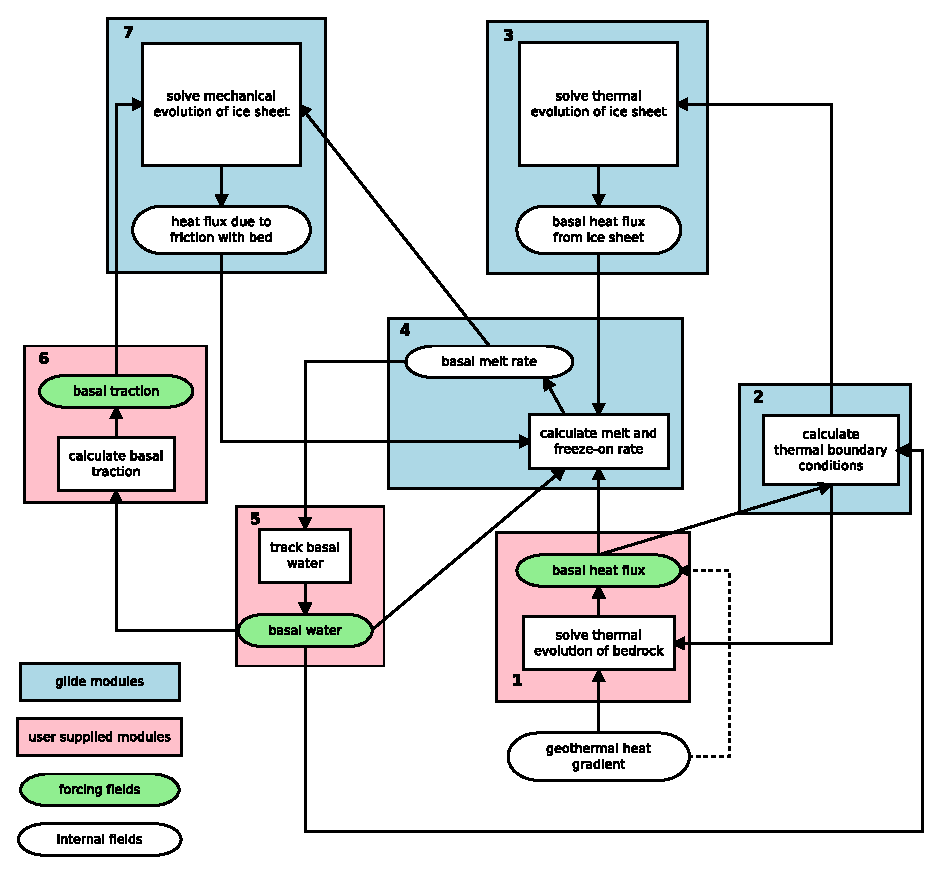
\includegraphics[width=\textwidth]{\dir/figs/basal_alg.eps}
  \caption{Flow diagram illustrating how the various modules communicate with each other by exchanging data fields.}
  \label{num.fig.bc_flow}
\end{figure}
The order of executions is then:
\begin{enumerate}
\item Find the basal heat flux by either solving the equation describing the thermal evolution of the lithosphere, \eqref{num.eq.diffu_rock}, or by using the geothermal heat flux directly. The upper boundary condition of \eqref{num.eq.diffu_rock} is the same as the lower boundary condition of the thermal evolution of the ice sheet.
\item Either (1) the lower boundary condition for the thermal evolution of the ice sheet is given by the basal heat flux from \emph{Step 1}; or (2) if melt water is present, the basal temperature is set to the pressure melting point of ice.
\item Calculate the temperature distribution within the ice sheet given the boundary condition found during \emph{Step 2} and the atmospheric BC.
\item Calculate a melt/freeze--on rate using Equation \eqref{bc.eq.meltrate} given the outgoing heat flux calculated during \emph{Step 3}, friction with the bed (calculated during the previous \emph{Step 7}) and the incoming heat flux from \emph{Step 1}. Freezing occurs only when there is basal water.
\item Track basal water. This is a user supplied module which can take any complexity. Inputs will typically be the melt/freeze--on rate determined during \emph{Step 4}.
\item Calculate the basal traction parameter. Again, this is a user supplied module which typically will involve the presence of basal water (calculated during \emph{Step 5}).
\item Solve the mechanical ice equations given basal traction parameter from \emph{Step 6}.
\end{enumerate}
Clearly, this scheme has the problem that heat is lost if the basal heat flux is such that more water could be frozen than is available. This might be avoided by iterating the process. On the other hand, the heat loss may be negligible if time steps are fairly small.
